\documentclass[12pt,a4paper]{scrartcl}\usepackage[]{graphicx}\usepackage[]{color}
%% maxwidth is the original width if it is less than linewidth
%% otherwise use linewidth (to make sure the graphics do not exceed the margin)
\makeatletter
\def\maxwidth{ %
  \ifdim\Gin@nat@width>\linewidth
    \linewidth
  \else
    \Gin@nat@width
  \fi
}
\makeatother

\definecolor{fgcolor}{rgb}{0.345, 0.345, 0.345}
\newcommand{\hlnum}[1]{\textcolor[rgb]{0.686,0.059,0.569}{#1}}%
\newcommand{\hlstr}[1]{\textcolor[rgb]{0.192,0.494,0.8}{#1}}%
\newcommand{\hlcom}[1]{\textcolor[rgb]{0.678,0.584,0.686}{\textit{#1}}}%
\newcommand{\hlopt}[1]{\textcolor[rgb]{0,0,0}{#1}}%
\newcommand{\hlstd}[1]{\textcolor[rgb]{0.345,0.345,0.345}{#1}}%
\newcommand{\hlkwa}[1]{\textcolor[rgb]{0.161,0.373,0.58}{\textbf{#1}}}%
\newcommand{\hlkwb}[1]{\textcolor[rgb]{0.69,0.353,0.396}{#1}}%
\newcommand{\hlkwc}[1]{\textcolor[rgb]{0.333,0.667,0.333}{#1}}%
\newcommand{\hlkwd}[1]{\textcolor[rgb]{0.737,0.353,0.396}{\textbf{#1}}}%
\let\hlipl\hlkwb

\usepackage{framed}
\makeatletter
\newenvironment{kframe}{%
 \def\at@end@of@kframe{}%
 \ifinner\ifhmode%
  \def\at@end@of@kframe{\end{minipage}}%
  \begin{minipage}{\columnwidth}%
 \fi\fi%
 \def\FrameCommand##1{\hskip\@totalleftmargin \hskip-\fboxsep
 \colorbox{shadecolor}{##1}\hskip-\fboxsep
     % There is no \\@totalrightmargin, so:
     \hskip-\linewidth \hskip-\@totalleftmargin \hskip\columnwidth}%
 \MakeFramed {\advance\hsize-\width
   \@totalleftmargin\z@ \linewidth\hsize
   \@setminipage}}%
 {\par\unskip\endMakeFramed%
 \at@end@of@kframe}
\makeatother

\definecolor{shadecolor}{rgb}{.97, .97, .97}
\definecolor{messagecolor}{rgb}{0, 0, 0}
\definecolor{warningcolor}{rgb}{1, 0, 1}
\definecolor{errorcolor}{rgb}{1, 0, 0}
\newenvironment{knitrout}{}{} % an empty environment to be redefined in TeX

\usepackage{alltt}
\usepackage[utf8]{inputenc}
\usepackage{amsmath}
\usepackage{graphicx}
\usepackage{tikz}
%\usepackage{silence}
\usepackage{mdframed}
%\WarningFilter{mdframed}{You got a bad break}
\usepackage[colorinlistoftodos]{todonotes}
\usepackage{listings}
\usepackage{color}
\colorlet{exampcol}{blue!10}
\usepackage{multicol}
\usepackage{booktabs}

\usepackage[noanswer]{exercise}%[noanswer]

\usepackage[autostyle, english = american]{csquotes}
\MakeOuterQuote{"}

\usepackage{hyperref}
\hypersetup{
    colorlinks,
    citecolor=black,
    filecolor=black,
    linkcolor=blue,
    urlcolor=black
}

\title{Exercises for linear mixed effect models, part 3}
\date{\today}
\author{Timoth\'ee Bonnet}
\IfFileExists{upquote.sty}{\usepackage{upquote}}{}
\begin{document}



\maketitle

\tableofcontents
\ListOfExerciseInToc
\ExerciseLevelInToc{subsubsection}

\clearpage 



\section{Logistic regression basics}

\begin{Exercise}[difficulty=1, title={Fit with glm()}]
Load the dataset \texttt{survivalsize.csv}. It contains fake data of individual-based measurements of body size and of survival from the time of measurement to the next year. Look at a summary of the data and plot them. Do you think size affects survival?
Use the function glm() to fit a logistic regression. What should the \texttt{family} argument be? What is the direction of the effect of size on survival?
\end{Exercise}
\begin{Answer}
\begin{knitrout}
\definecolor{shadecolor}{rgb}{0.969, 0.969, 0.969}\color{fgcolor}\begin{kframe}
\begin{alltt}
\hlstd{survdat} \hlkwb{<-} \hlkwd{read.csv}\hlstd{(}\hlstr{"survivalsize.csv"}\hlstd{)}
\hlkwd{summary}\hlstd{(survdat)}
\end{alltt}
\begin{verbatim}
##     survival          size     
##  Min.   :0.000   Min.   :2.69  
##  1st Qu.:0.000   1st Qu.:4.37  
##  Median :1.000   Median :4.94  
##  Mean   :0.555   Mean   :4.99  
##  3rd Qu.:1.000   3rd Qu.:5.57  
##  Max.   :1.000   Max.   :8.24
\end{verbatim}
\begin{alltt}
\hlkwd{plot}\hlstd{(survdat)}
\end{alltt}
\end{kframe}
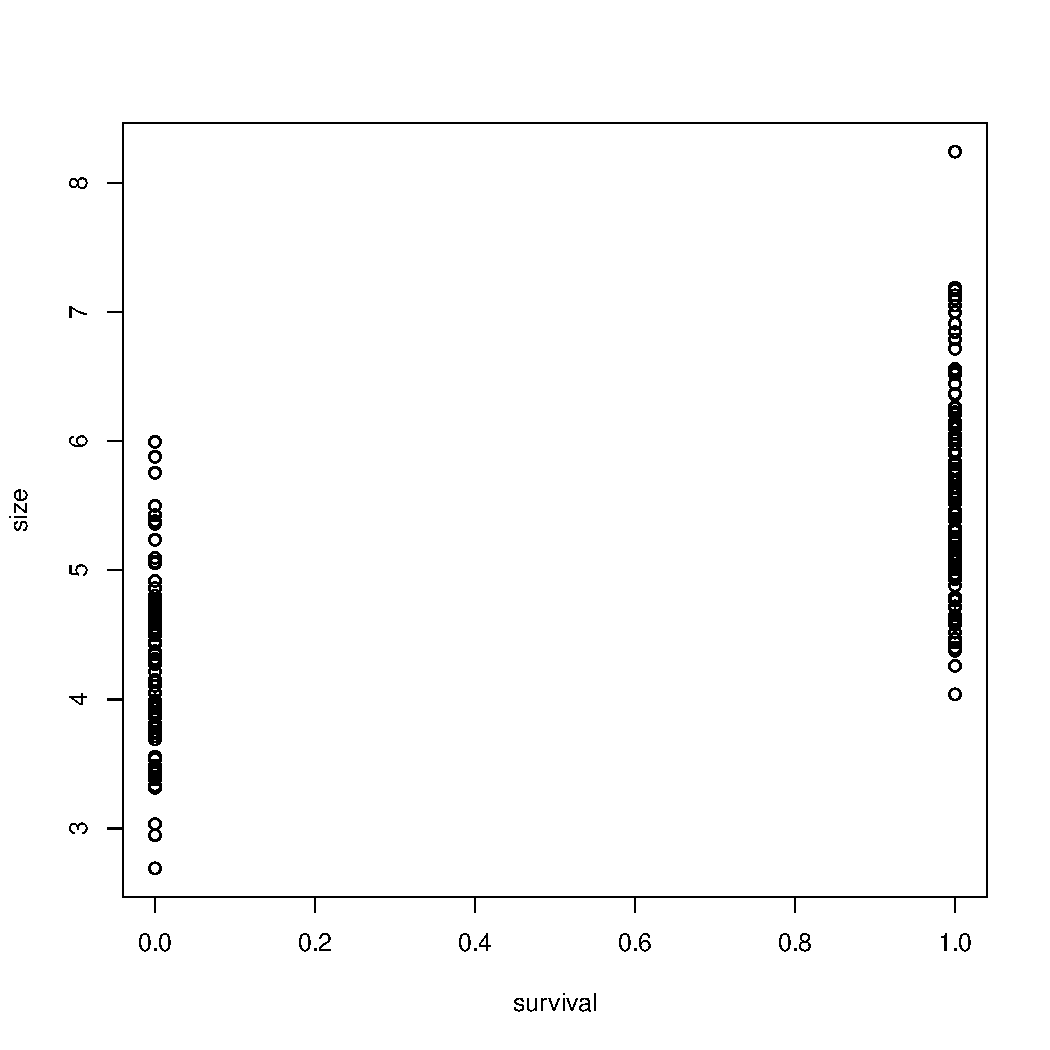
\includegraphics[width=\maxwidth]{figure/unnamed-chunk-2-1} 
\begin{kframe}\begin{alltt}
\hlstd{glmsurvsize0} \hlkwb{<-} \hlkwd{glm}\hlstd{(survival} \hlopt{~} \hlnum{1} \hlopt{+} \hlstd{size,} \hlkwc{data} \hlstd{= survdat,}
                    \hlkwc{family} \hlstd{=} \hlstr{"binomial"}\hlstd{)}
\hlkwd{summary}\hlstd{(glmsurvsize0)}
\end{alltt}
\begin{verbatim}
## 
## Call:
## glm(formula = survival ~ 1 + size, family = "binomial", data = survdat)
## 
## Deviance Residuals: 
##    Min      1Q  Median      3Q     Max  
## -2.602  -0.606   0.108   0.641   2.122  
## 
## Coefficients:
##             Estimate Std. Error z value Pr(>|z|)    
## (Intercept)  -13.478      1.949   -6.92  4.6e-12 ***
## size           2.808      0.402    6.99  2.7e-12 ***
## ---
## Signif. codes:  0 '***' 0.001 '**' 0.01 '*' 0.05 '.' 0.1 ' ' 1
## 
## (Dispersion parameter for binomial family taken to be 1)
## 
##     Null deviance: 274.83  on 199  degrees of freedom
## Residual deviance: 159.02  on 198  degrees of freedom
## AIC: 163
## 
## Number of Fisher Scoring iterations: 6
\end{verbatim}
\end{kframe}
\end{knitrout}
\end{Answer}

\begin{Exercise}[difficulty=1, title={Model assumptions}]
In R some model assumptions of linear models are routinely checked using plot(lm()): residual normality, independance and homogeneous variance, and legerage. If you know about these diagnostics (and what the plots should ideally look like) check them for your glm. Should you worry?
\end{Exercise}
\begin{Answer}
\begin{knitrout}
\definecolor{shadecolor}{rgb}{0.969, 0.969, 0.969}\color{fgcolor}\begin{kframe}
\begin{alltt}
\hlkwd{plot}\hlstd{(glmsurvsize0)}
\end{alltt}
\end{kframe}
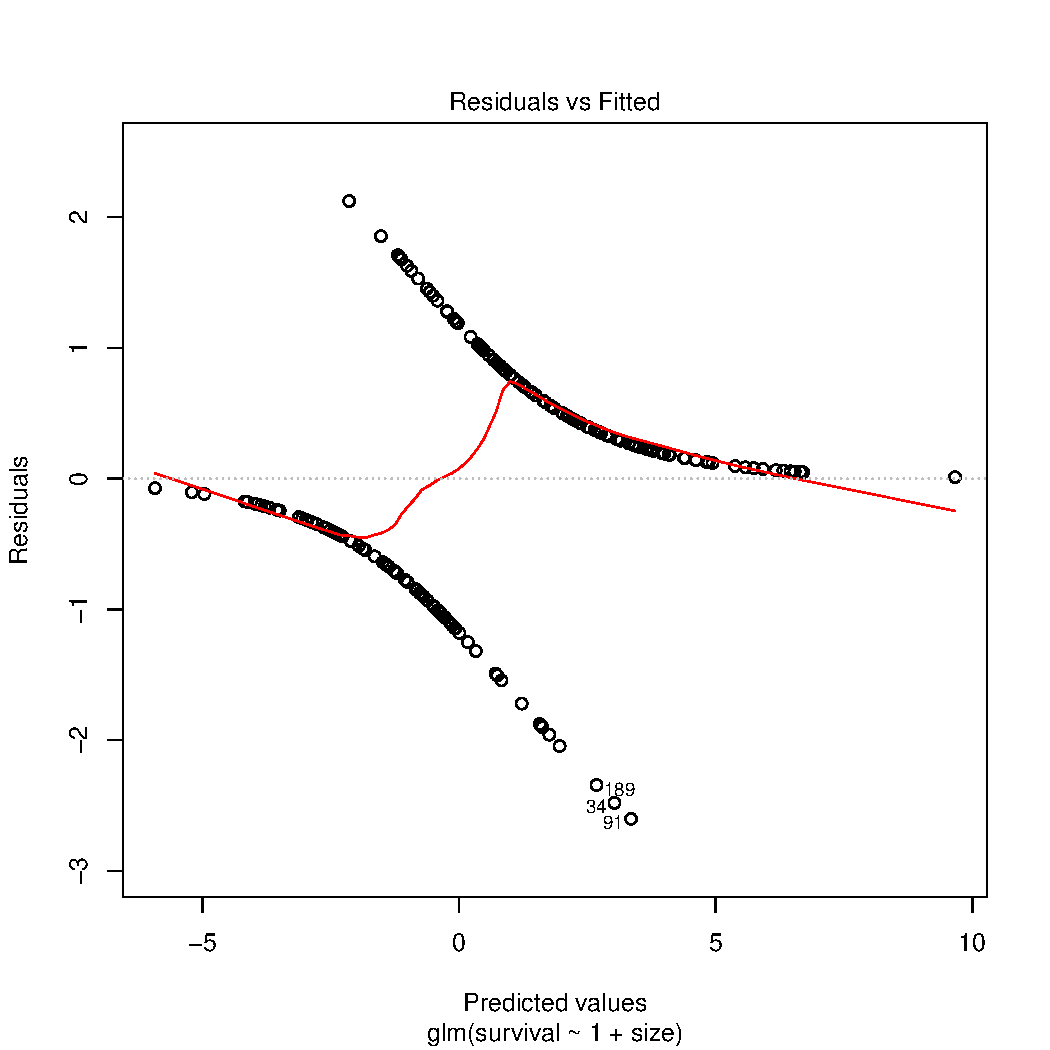
\includegraphics[width=\maxwidth]{figure/unnamed-chunk-3-1} 

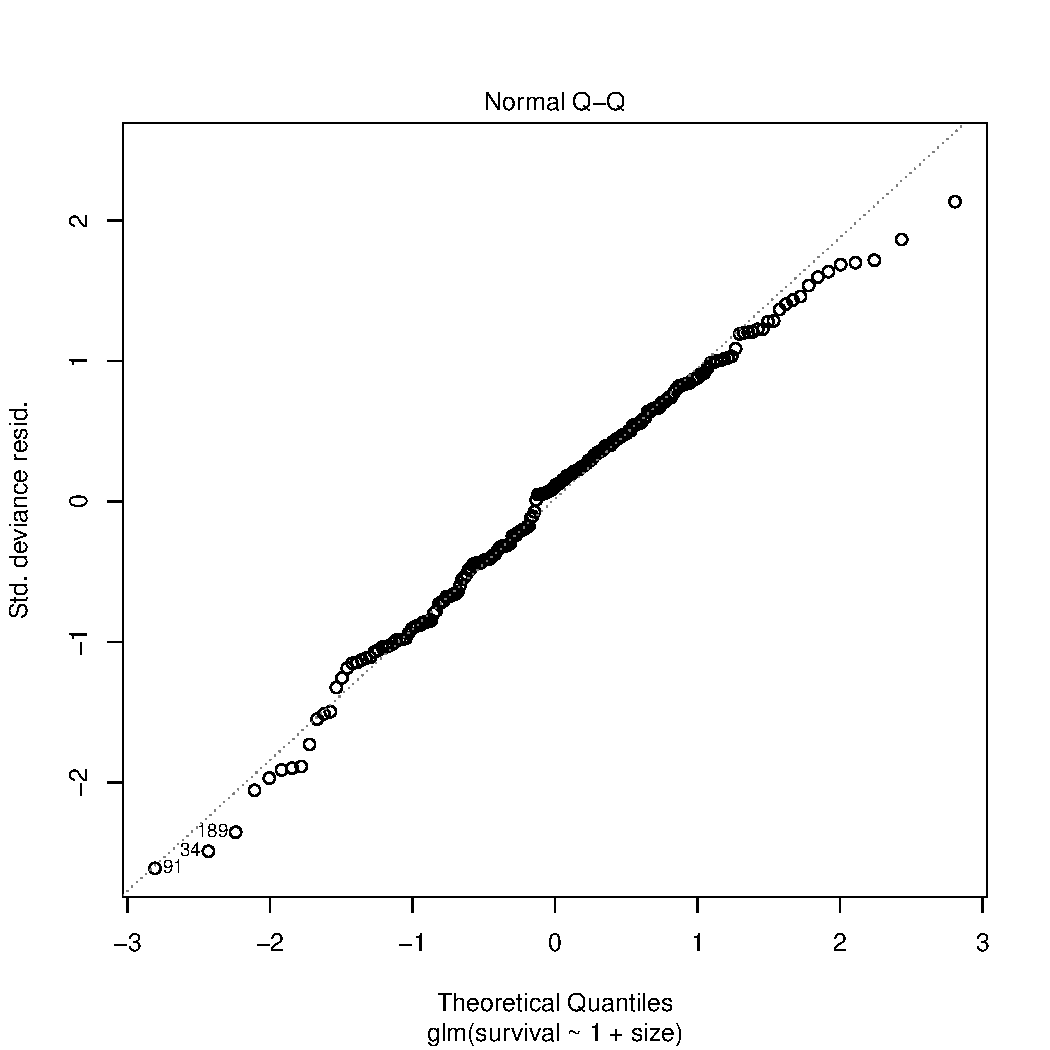
\includegraphics[width=\maxwidth]{figure/unnamed-chunk-3-2} 

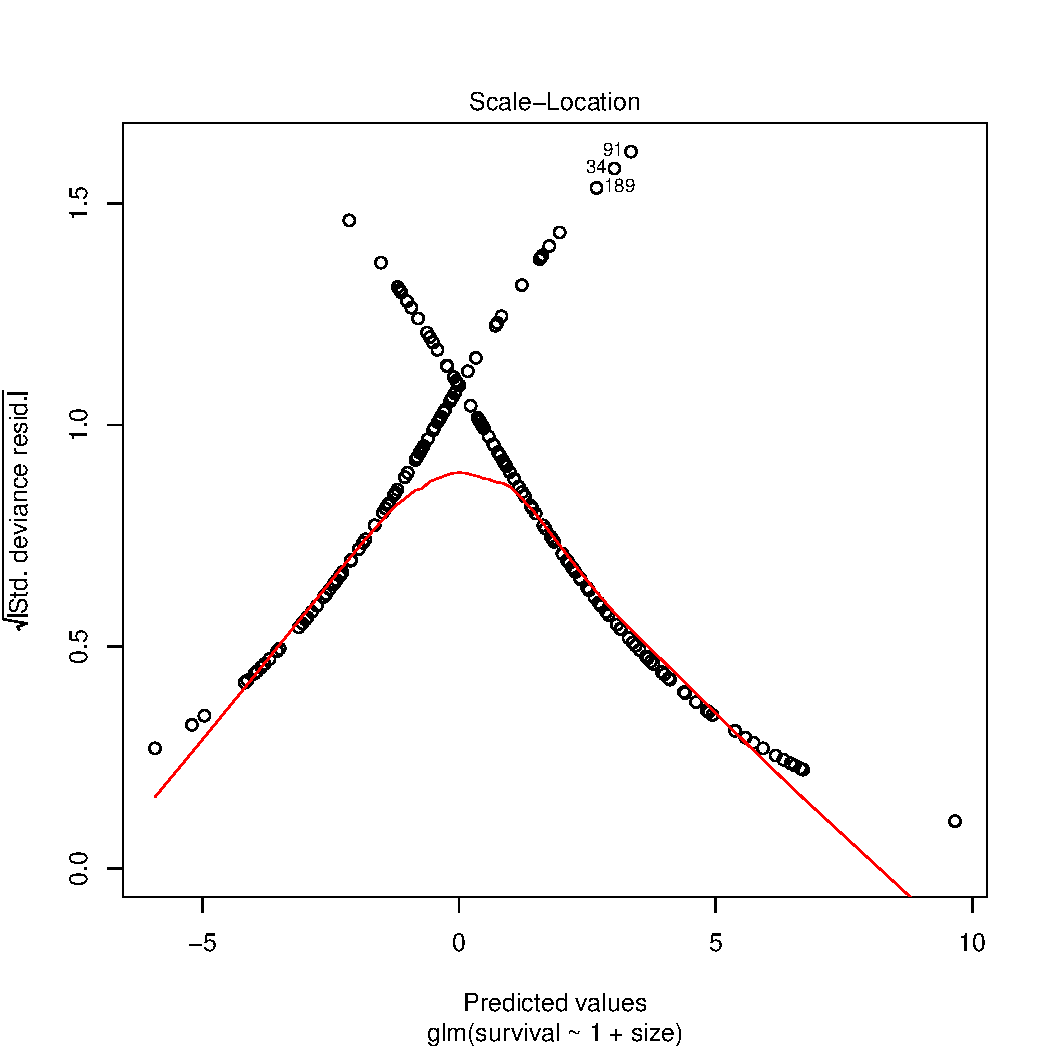
\includegraphics[width=\maxwidth]{figure/unnamed-chunk-3-3} 

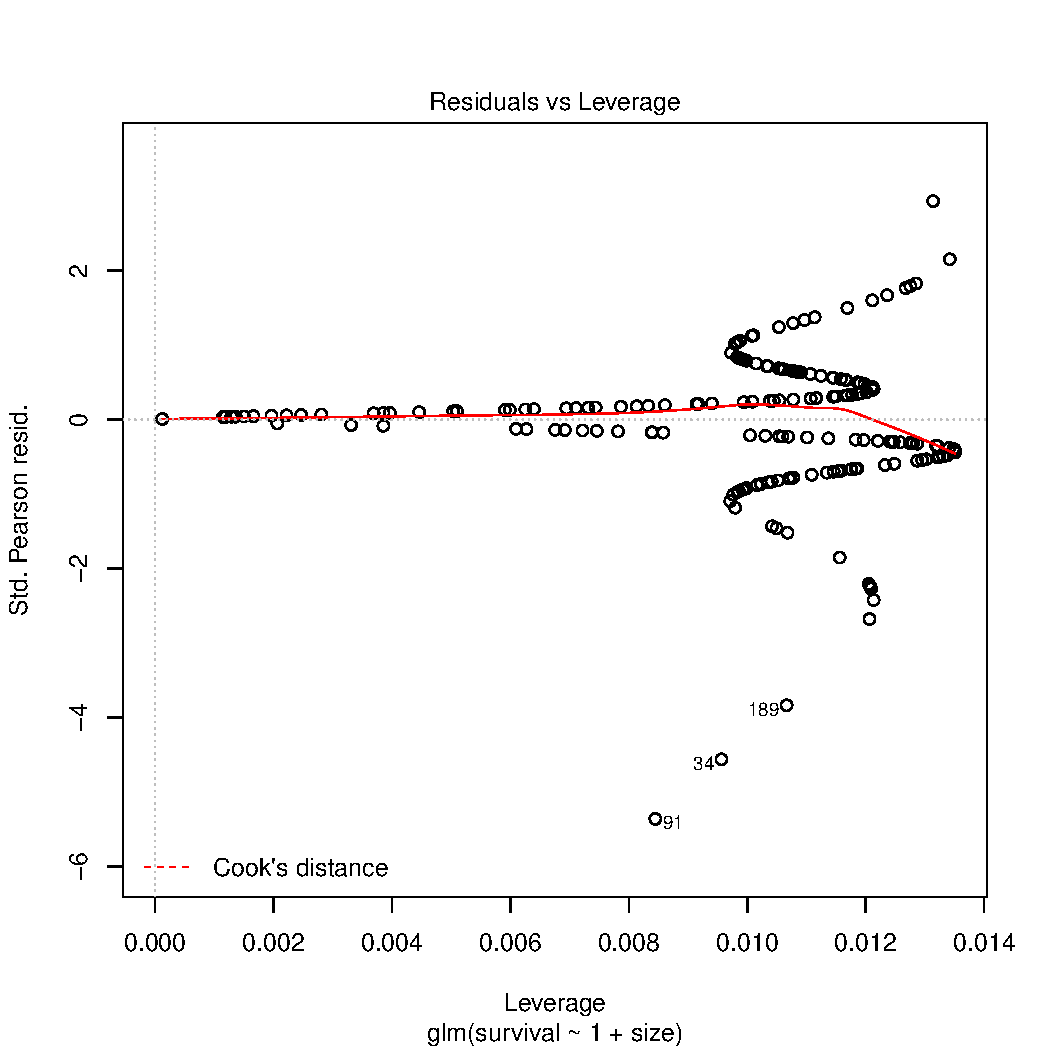
\includegraphics[width=\maxwidth]{figure/unnamed-chunk-3-4} 

\end{knitrout}
No. A binary logistic regression makes much less stringent assumptions than a linear model. The one thing you can easily check if that data are binary. The assumptions that may be violated (non-independance and no measurement error) would generally not be visible on these plots. The definition of a logistic regression means that the residuals will generally not follow a normal distribution, but will be dependent on the predictors, and will have changing variance; that is perfectly okay.
\end{Answer}

\begin{Exercise}[difficulty=2, title={Making sense of model estimates}]
Consider the model estimates for the intercept and slope.  How to recover the mean survival from these two numbers? You will need to use the back-transformation inverse logit: probability = $\frac{1}{1+\exp(-y)}$ where $y$ is a model prediction on the logit-scale. You can also use the function \texttt{predict()}.

How much does the ratio of surviving/dying probabilities changes for an individual of size 6 compared to an individual of size 5?
\end{Exercise}
\begin{Answer}
\begin{knitrout}
\definecolor{shadecolor}{rgb}{0.969, 0.969, 0.969}\color{fgcolor}\begin{kframe}
\begin{alltt}
\hlkwd{summary}\hlstd{(glmsurvsize0)}
\end{alltt}
\begin{verbatim}
## 
## Call:
## glm(formula = survival ~ 1 + size, family = "binomial", data = survdat)
## 
## Deviance Residuals: 
##    Min      1Q  Median      3Q     Max  
## -2.602  -0.606   0.108   0.641   2.122  
## 
## Coefficients:
##             Estimate Std. Error z value Pr(>|z|)    
## (Intercept)  -13.478      1.949   -6.92  4.6e-12 ***
## size           2.808      0.402    6.99  2.7e-12 ***
## ---
## Signif. codes:  0 '***' 0.001 '**' 0.01 '*' 0.05 '.' 0.1 ' ' 1
## 
## (Dispersion parameter for binomial family taken to be 1)
## 
##     Null deviance: 274.83  on 199  degrees of freedom
## Residual deviance: 159.02  on 198  degrees of freedom
## AIC: 163
## 
## Number of Fisher Scoring iterations: 6
\end{verbatim}
\end{kframe}
\end{knitrout}

The data mean survival is:
\begin{knitrout}
\definecolor{shadecolor}{rgb}{0.969, 0.969, 0.969}\color{fgcolor}\begin{kframe}
\begin{alltt}
\hlkwd{mean}\hlstd{(survdat}\hlopt{$}\hlstd{survival)}
\end{alltt}
\begin{verbatim}
## [1] 0.555
\end{verbatim}
\end{kframe}
\end{knitrout}

You CANNOT recover the mean data survival by back-transforming the predicted mean on the logit-scale, because the back-transformation is not linear:
\begin{knitrout}
\definecolor{shadecolor}{rgb}{0.969, 0.969, 0.969}\color{fgcolor}\begin{kframe}
\begin{alltt}
\hlstd{meanlogit} \hlkwb{<-} \hlkwd{mean}\hlstd{(}\hlkwd{coefficients}\hlstd{(glmsurvsize0)[}\hlnum{1}\hlstd{]}\hlopt{+}
\hlkwd{coefficients}\hlstd{(glmsurvsize0)[}\hlnum{2}\hlstd{]}\hlopt{*}\hlstd{survdat}\hlopt{$}\hlstd{size)}

\hlnum{1}\hlopt{/}\hlstd{(}\hlnum{1}\hlopt{+}\hlkwd{exp}\hlstd{(}\hlopt{-}\hlstd{meanlogit))}
\end{alltt}
\begin{verbatim}
## [1] 0.6311
\end{verbatim}
\end{kframe}
\end{knitrout}

You must back-transform individual data points and THEN calculate the mean:
\begin{knitrout}
\definecolor{shadecolor}{rgb}{0.969, 0.969, 0.969}\color{fgcolor}\begin{kframe}
\begin{alltt}
\hlstd{preddat} \hlkwb{<-} \hlkwd{coefficients}\hlstd{(glmsurvsize0)[}\hlnum{1}\hlstd{]}\hlopt{+}
\hlkwd{coefficients}\hlstd{(glmsurvsize0)[}\hlnum{2}\hlstd{]}\hlopt{*}\hlstd{(survdat}\hlopt{$}\hlstd{size)}
\hlkwd{mean}\hlstd{(}\hlnum{1}\hlopt{/}\hlstd{(}\hlnum{1}\hlopt{+}\hlkwd{exp}\hlstd{(}\hlopt{-}\hlstd{preddat)))}
\end{alltt}
\begin{verbatim}
## [1] 0.555
\end{verbatim}
\end{kframe}
\end{knitrout}
The function predict with \texttt{type} argument set to \texttt{response} can help with the back-transformation:
\begin{knitrout}
\definecolor{shadecolor}{rgb}{0.969, 0.969, 0.969}\color{fgcolor}\begin{kframe}
\begin{alltt}
\hlkwd{mean}\hlstd{(}\hlkwd{predict}\hlstd{(glmsurvsize0,} \hlkwc{type} \hlstd{=} \hlstr{"response"}\hlstd{))}
\end{alltt}
\begin{verbatim}
## [1] 0.555
\end{verbatim}
\end{kframe}
\end{knitrout}

The increase in the odd survive with an increase of one unit in size is an odd-ratio. It is simply the exponential of the slope:
\begin{knitrout}
\definecolor{shadecolor}{rgb}{0.969, 0.969, 0.969}\color{fgcolor}\begin{kframe}
\begin{alltt}
\hlkwd{exp}\hlstd{(}\hlkwd{coefficients}\hlstd{(glmsurvsize0)[}\hlnum{2}\hlstd{])}
\end{alltt}
\begin{verbatim}
##  size 
## 16.57
\end{verbatim}
\end{kframe}
\end{knitrout}

You can check this by comparing two predictions
\begin{knitrout}
\definecolor{shadecolor}{rgb}{0.969, 0.969, 0.969}\color{fgcolor}\begin{kframe}
\begin{alltt}
\hlstd{survprob5} \hlkwb{<-} \hlnum{1}\hlopt{/}\hlstd{(}\hlnum{1}\hlopt{+}\hlkwd{exp}\hlstd{(}\hlopt{-}\hlstd{(}\hlkwd{coefficients}\hlstd{(glmsurvsize0)[}\hlnum{1}\hlstd{]}\hlopt{+}
                          \hlnum{5}\hlopt{*}\hlkwd{coefficients}\hlstd{(glmsurvsize0)[}\hlnum{2}\hlstd{])))}
\hlstd{survprob6} \hlkwb{<-} \hlnum{1}\hlopt{/}\hlstd{(}\hlnum{1}\hlopt{+}\hlkwd{exp}\hlstd{(}\hlopt{-}\hlstd{(}\hlkwd{coefficients}\hlstd{(glmsurvsize0)[}\hlnum{1}\hlstd{]}\hlopt{+}
                          \hlnum{6}\hlopt{*}\hlkwd{coefficients}\hlstd{(glmsurvsize0)[}\hlnum{2}\hlstd{])))}

\hlcom{#definition of odd-ratio:}
\hlstd{(survprob6}\hlopt{/}\hlstd{(}\hlnum{1}\hlopt{-}\hlstd{survprob6))}\hlopt{/}\hlstd{(survprob5}\hlopt{/}\hlstd{(}\hlnum{1}\hlopt{-}\hlstd{survprob5))}
\end{alltt}
\begin{verbatim}
## (Intercept) 
##       16.57
\end{verbatim}
\end{kframe}
\end{knitrout}

\end{Answer}

\begin{Exercise}[difficulty=2, title={Visualize results}]
Use the function \texttt{predict()} to make a graph of the relationship between survival and size, with a confidence interval. 
\end{Exercise}
\begin{Answer}
\begin{knitrout}
\definecolor{shadecolor}{rgb}{0.969, 0.969, 0.969}\color{fgcolor}\begin{kframe}
\begin{alltt}
\hlkwd{plot}\hlstd{(survdat}\hlopt{$}\hlstd{size, survdat}\hlopt{$}\hlstd{survival,} \hlkwc{xlab}\hlstd{=}\hlstr{"Size"}\hlstd{,} \hlkwc{ylab}\hlstd{=}\hlstr{"Survival"}\hlstd{)}

\hlstd{newdat} \hlkwb{<-} \hlkwd{data.frame}\hlstd{(}\hlkwc{size}\hlstd{=}\hlkwd{seq}\hlstd{(}\hlkwd{min}\hlstd{(survdat}\hlopt{$}\hlstd{size),}\hlkwd{max}\hlstd{(survdat}\hlopt{$}\hlstd{size),}
                              \hlkwc{length.out} \hlstd{=} \hlnum{100}\hlstd{))}
\hlstd{newdat} \hlkwb{<-} \hlkwd{cbind}\hlstd{(newdat,} \hlkwd{predict}\hlstd{(glmsurvsize0,} \hlkwc{newdata} \hlstd{= newdat,}
                                \hlkwc{type} \hlstd{=} \hlstr{"link"}\hlstd{,} \hlkwc{se.fit} \hlstd{=} \hlnum{TRUE}\hlstd{))}
\hlstd{newdat}\hlopt{$}\hlstd{ciu} \hlkwb{<-} \hlnum{1}\hlopt{/}\hlstd{(}\hlnum{1}\hlopt{+}\hlkwd{exp}\hlstd{(}\hlopt{-}\hlstd{(newdat}\hlopt{$}\hlstd{fit} \hlopt{+} \hlnum{1.96}\hlopt{*}\hlstd{newdat}\hlopt{$}\hlstd{se.fit)))}
\hlstd{newdat}\hlopt{$}\hlstd{cil} \hlkwb{<-} \hlnum{1}\hlopt{/}\hlstd{(}\hlnum{1}\hlopt{+}\hlkwd{exp}\hlstd{(}\hlopt{-}\hlstd{(newdat}\hlopt{$}\hlstd{fit} \hlopt{-} \hlnum{1.96}\hlopt{*}\hlstd{newdat}\hlopt{$}\hlstd{se.fit)))}
\hlstd{newdat}\hlopt{$}\hlstd{prob} \hlkwb{<-} \hlnum{1}\hlopt{/}\hlstd{(}\hlnum{1}\hlopt{+}\hlkwd{exp}\hlstd{(}\hlopt{-}\hlstd{(newdat}\hlopt{$}\hlstd{fit)))}

\hlkwd{lines}\hlstd{(}\hlkwc{x} \hlstd{= newdat}\hlopt{$}\hlstd{size, newdat}\hlopt{$}\hlstd{prob,} \hlkwc{lwd}\hlstd{=}\hlnum{5}\hlstd{,} \hlkwc{col}\hlstd{=}\hlstr{'red'}\hlstd{)}
\hlcom{#confidence interval with lines}
\hlkwd{lines}\hlstd{(}\hlkwc{x} \hlstd{= newdat}\hlopt{$}\hlstd{size, newdat}\hlopt{$}\hlstd{ciu,} \hlkwc{lwd}\hlstd{=}\hlnum{3}\hlstd{,} \hlkwc{col}\hlstd{=}\hlstr{'red'}\hlstd{,} \hlkwc{lty}\hlstd{=}\hlnum{2}\hlstd{)}
\hlkwd{lines}\hlstd{(}\hlkwc{x} \hlstd{= newdat}\hlopt{$}\hlstd{size, newdat}\hlopt{$}\hlstd{cil,} \hlkwc{lwd}\hlstd{=}\hlnum{3}\hlstd{,} \hlkwc{col}\hlstd{=}\hlstr{'red'}\hlstd{,} \hlkwc{lty}\hlstd{=}\hlnum{2}\hlstd{)}

\hlcom{#or with polygon:}
\hlkwd{polygon}\hlstd{(}\hlkwc{x}\hlstd{=}\hlkwd{c}\hlstd{(newdat}\hlopt{$}\hlstd{size,}\hlkwd{rev}\hlstd{(newdat}\hlopt{$}\hlstd{size)),}
        \hlkwc{y}\hlstd{=}\hlkwd{c}\hlstd{(newdat}\hlopt{$}\hlstd{ciu,}\hlkwd{rev}\hlstd{(newdat}\hlopt{$}\hlstd{cil)),}
        \hlkwc{col} \hlstd{=} \hlkwd{rgb}\hlstd{(}\hlnum{0.8}\hlstd{,}\hlnum{0}\hlstd{,}\hlnum{0}\hlstd{,}\hlnum{0.2}\hlstd{),} \hlkwc{border} \hlstd{=}\hlnum{NA}\hlstd{)}
\end{alltt}
\end{kframe}
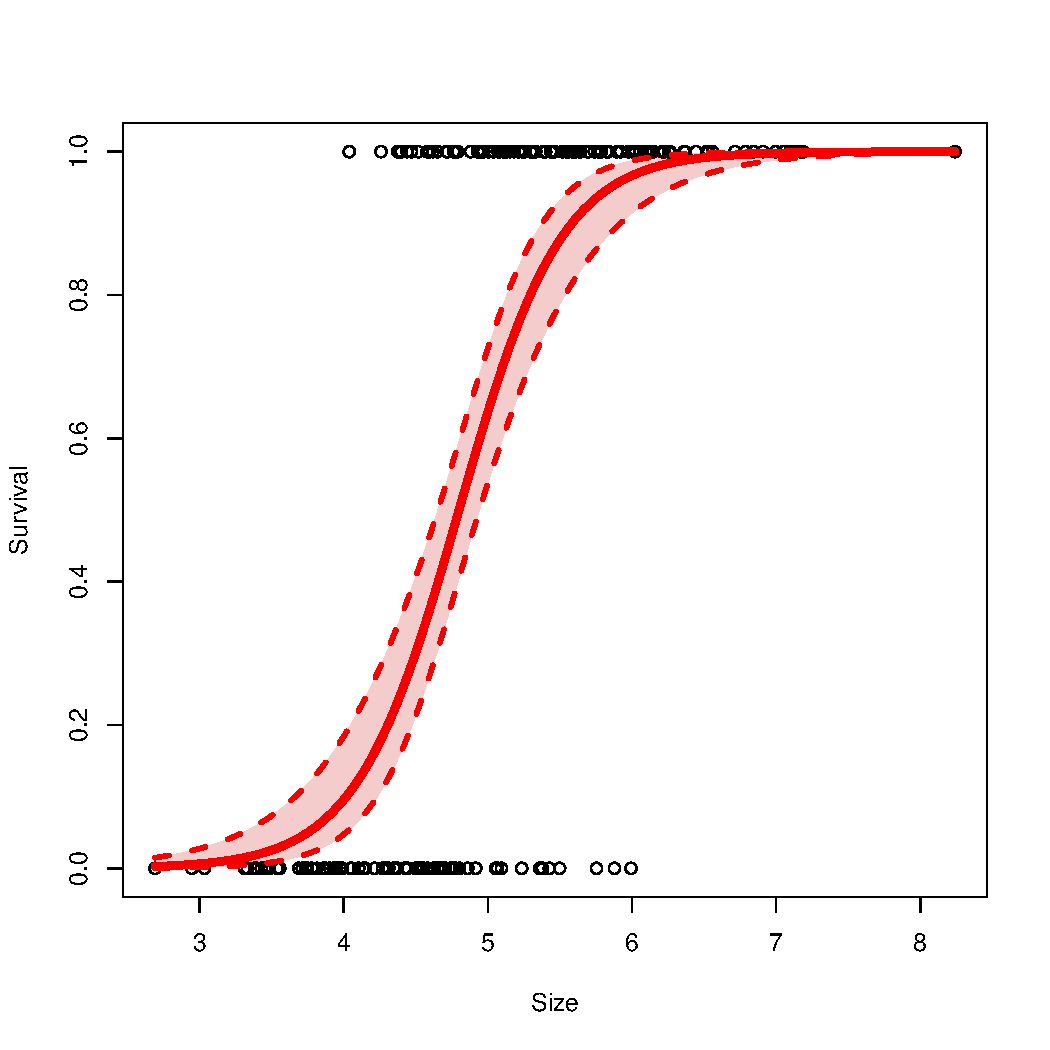
\includegraphics[width=\maxwidth]{figure/unnamed-chunk-11-1} 

\end{knitrout}
\end{Answer}



\section{Classification}

\begin{Exercise}[difficulty=2, title={What populations are at risk?}]
Researchers are currently trying to predict animal population collapses in advance, by finding metrics that changed before historic populations collapsed. Let's imagine we have measured the time-autocorrelation in phenotypes (what that means does not matter) in 200 populations, some of which have collapsed in the past decades. We want to konw whether autocorrelation is related to collapse, and whether it could be used to predict which population will collapse in the future. 

Load the dataset \texttt{decline.csv}, it contains fake data of past collapses and past autocorrelations in populations, as well as future collapses (yes, I am a fortune teller). Fit a logistic regression of \texttt{popcollapse} as a function of \texttt{atcor}. Does \texttt{atcor} increase the probability of population collapse? Visualize the relationship. Does it make sense to define a threshold of autocorrelation and allocate conservation resources to those populations that are at risk based on our metric? For instance, what do you think about conserving all populations above an autocorrelation of 0.5? How many future at-risk populations would be missed? How many populations that are not at risk would receive unecessary resources? How could you improve the prediction?


\end{Exercise}
\begin{Answer}
\begin{knitrout}
\definecolor{shadecolor}{rgb}{0.969, 0.969, 0.969}\color{fgcolor}\begin{kframe}
\begin{alltt}
\hlstd{decline} \hlkwb{<-} \hlkwd{read.csv}\hlstd{(}\hlstr{"decline.csv"}\hlstd{)}
\hlkwd{summary}\hlstd{(glmcoll0} \hlkwb{<-} \hlkwd{glm}\hlstd{(popcollapse}\hlopt{~}\hlstd{pheno_autocorr,}
                      \hlkwc{data} \hlstd{= decline,} \hlkwc{family} \hlstd{=} \hlstr{"binomial"}\hlstd{))}
\end{alltt}
\begin{verbatim}
## 
## Call:
## glm(formula = popcollapse ~ pheno_autocorr, family = "binomial", 
##     data = decline)
## 
## Deviance Residuals: 
##    Min      1Q  Median      3Q     Max  
## -0.777  -0.611  -0.497  -0.429   2.196  
## 
## Coefficients:
##                Estimate Std. Error z value Pr(>|z|)    
## (Intercept)      -1.772      0.206   -8.61   <2e-16 ***
## pheno_autocorr    0.732      0.353    2.07    0.038 *  
## ---
## Signif. codes:  0 '***' 0.001 '**' 0.01 '*' 0.05 '.' 0.1 ' ' 1
## 
## (Dispersion parameter for binomial family taken to be 1)
## 
##     Null deviance: 169.08  on 199  degrees of freedom
## Residual deviance: 164.64  on 198  degrees of freedom
## AIC: 168.6
## 
## Number of Fisher Scoring iterations: 4
\end{verbatim}
\begin{alltt}
\hlstd{newdat} \hlkwb{<-} \hlkwd{data.frame}\hlstd{(}\hlkwc{pheno_autocorr}\hlstd{=}\hlkwd{seq}\hlstd{(}\hlopt{-}\hlnum{1}\hlstd{,}\hlnum{1}\hlstd{,}\hlkwc{length.out} \hlstd{=} \hlnum{100}\hlstd{))}
\hlstd{newdat} \hlkwb{<-} \hlkwd{cbind}\hlstd{(newdat,} \hlkwc{pred} \hlstd{=} \hlkwd{predict}\hlstd{(glmcoll0,}
                          \hlkwc{type} \hlstd{=} \hlstr{"response"}\hlstd{,} \hlkwc{newdata} \hlstd{= newdat))}

\hlkwd{plot}\hlstd{(decline}\hlopt{$}\hlstd{pheno_autocorr, decline}\hlopt{$}\hlstd{popcollapse)}
\hlkwd{lines}\hlstd{(newdat}\hlopt{$}\hlstd{pheno_autocorr, newdat}\hlopt{$}\hlstd{pred,} \hlkwc{col}\hlstd{=}\hlstr{"red"}\hlstd{)}
\end{alltt}
\end{kframe}
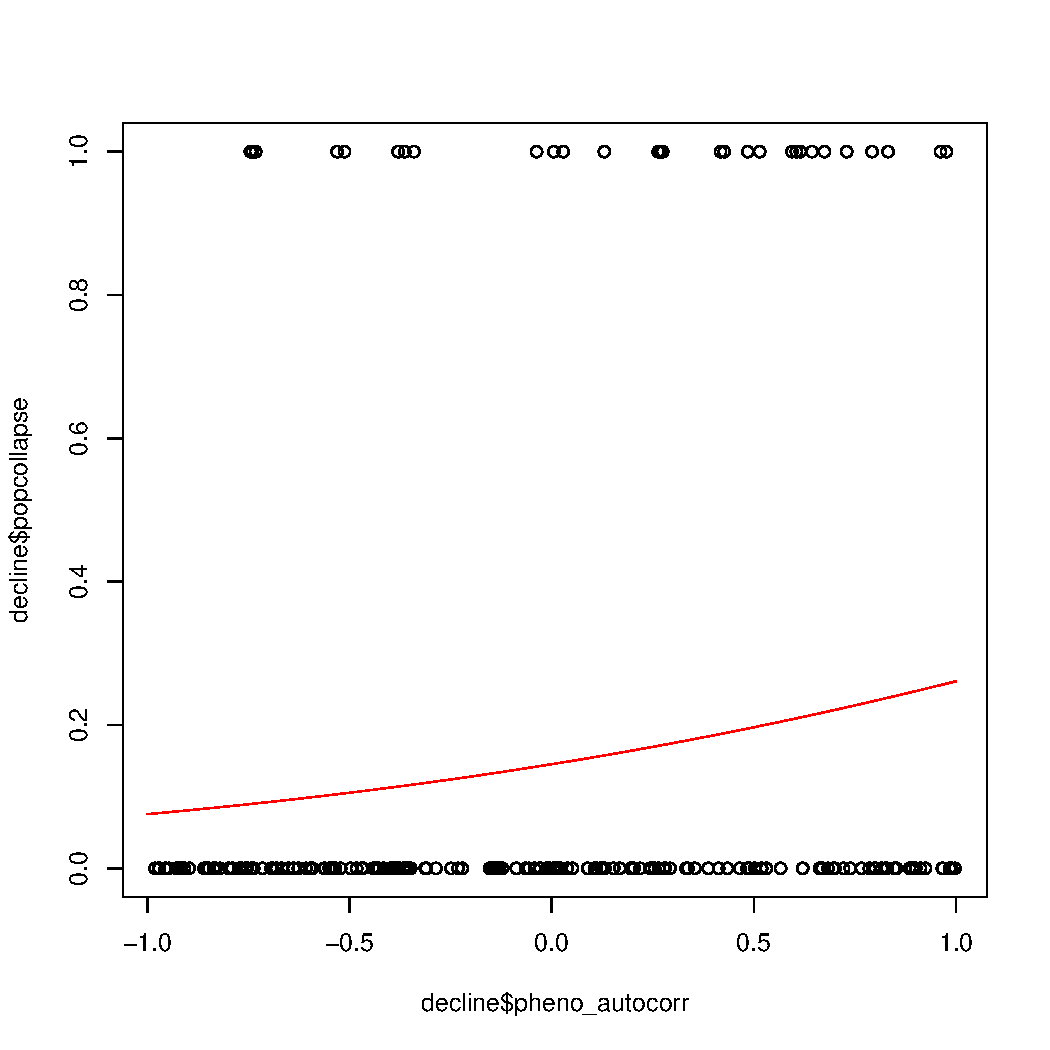
\includegraphics[width=\maxwidth]{figure/unnamed-chunk-13-1} 

\end{knitrout}

Using a threshold of 0.5 would be correct for 5 at-risk populations:
\begin{knitrout}
\definecolor{shadecolor}{rgb}{0.969, 0.969, 0.969}\color{fgcolor}\begin{kframe}
\begin{alltt}
\hlkwd{sum}\hlstd{(decline}\hlopt{$}\hlstd{futurecollapse[decline}\hlopt{$}\hlstd{pheno_autocorr}\hlopt{>=}\hlnum{0.5}\hlstd{],}
    \hlkwc{na.rm}\hlstd{=}\hlnum{TRUE}\hlstd{)}
\end{alltt}
\begin{verbatim}
## [1] 5
\end{verbatim}
\end{kframe}
\end{knitrout}

and 116 safe populations:
\begin{knitrout}
\definecolor{shadecolor}{rgb}{0.969, 0.969, 0.969}\color{fgcolor}\begin{kframe}
\begin{alltt}
\hlkwd{sum}\hlstd{(}\hlnum{1}\hlopt{-}\hlstd{decline}\hlopt{$}\hlstd{futurecollapse[decline}\hlopt{$}\hlstd{pheno_autocorr}\hlopt{<}\hlnum{0.5}\hlstd{],}
    \hlkwc{na.rm}\hlstd{=}\hlnum{TRUE}\hlstd{)}
\end{alltt}
\begin{verbatim}
## [1] 116
\end{verbatim}
\end{kframe}
\end{knitrout}

But would be incorrect for 19 at-risk populations and 30 safe populations:
\begin{knitrout}
\definecolor{shadecolor}{rgb}{0.969, 0.969, 0.969}\color{fgcolor}\begin{kframe}
\begin{alltt}
\hlkwd{sum}\hlstd{(decline}\hlopt{$}\hlstd{futurecollapse[decline}\hlopt{$}\hlstd{pheno_autocorr}\hlopt{<}\hlnum{0.5}\hlstd{],}
    \hlkwc{na.rm}\hlstd{=}\hlnum{TRUE}\hlstd{)}
\end{alltt}
\begin{verbatim}
## [1] 19
\end{verbatim}
\begin{alltt}
\hlkwd{sum}\hlstd{(}\hlnum{1}\hlopt{-}\hlstd{decline}\hlopt{$}\hlstd{futurecollapse[decline}\hlopt{$}\hlstd{pheno_autocorr}\hlopt{>=}\hlnum{0.5}\hlstd{],}
    \hlkwc{na.rm}\hlstd{=}\hlnum{TRUE}\hlstd{)}
\end{alltt}
\begin{verbatim}
## [1] 30
\end{verbatim}
\end{kframe}
\end{knitrout}

As could have been expected, this is a pretty bad performance. The result can be obtained more formally looking at a Receiver Operating Characteristic plot:
\begin{knitrout}
\definecolor{shadecolor}{rgb}{0.969, 0.969, 0.969}\color{fgcolor}\begin{kframe}
\begin{alltt}
\hlkwd{library}\hlstd{(pROC)} \hlcom{#need to install this package!}
\end{alltt}


{\ttfamily\noindent\itshape\color{messagecolor}{\#\# Type 'citation("{}pROC"{})' for a citation.}}

{\ttfamily\noindent\itshape\color{messagecolor}{\#\# \\\#\# Attaching package: 'pROC'}}

{\ttfamily\noindent\itshape\color{messagecolor}{\#\# The following objects are masked from 'package:stats':\\\#\# \\\#\#\ \ \ \  cov, smooth, var}}\begin{alltt}
\hlkwd{plot.roc}\hlstd{(}\hlkwc{predictor} \hlstd{=} \hlkwd{predict}\hlstd{(glmcoll0,} \hlkwc{type} \hlstd{=} \hlstr{"response"}\hlstd{),}
         \hlkwc{x} \hlstd{= decline}\hlopt{$}\hlstd{popcollapse)}
\end{alltt}
\end{kframe}
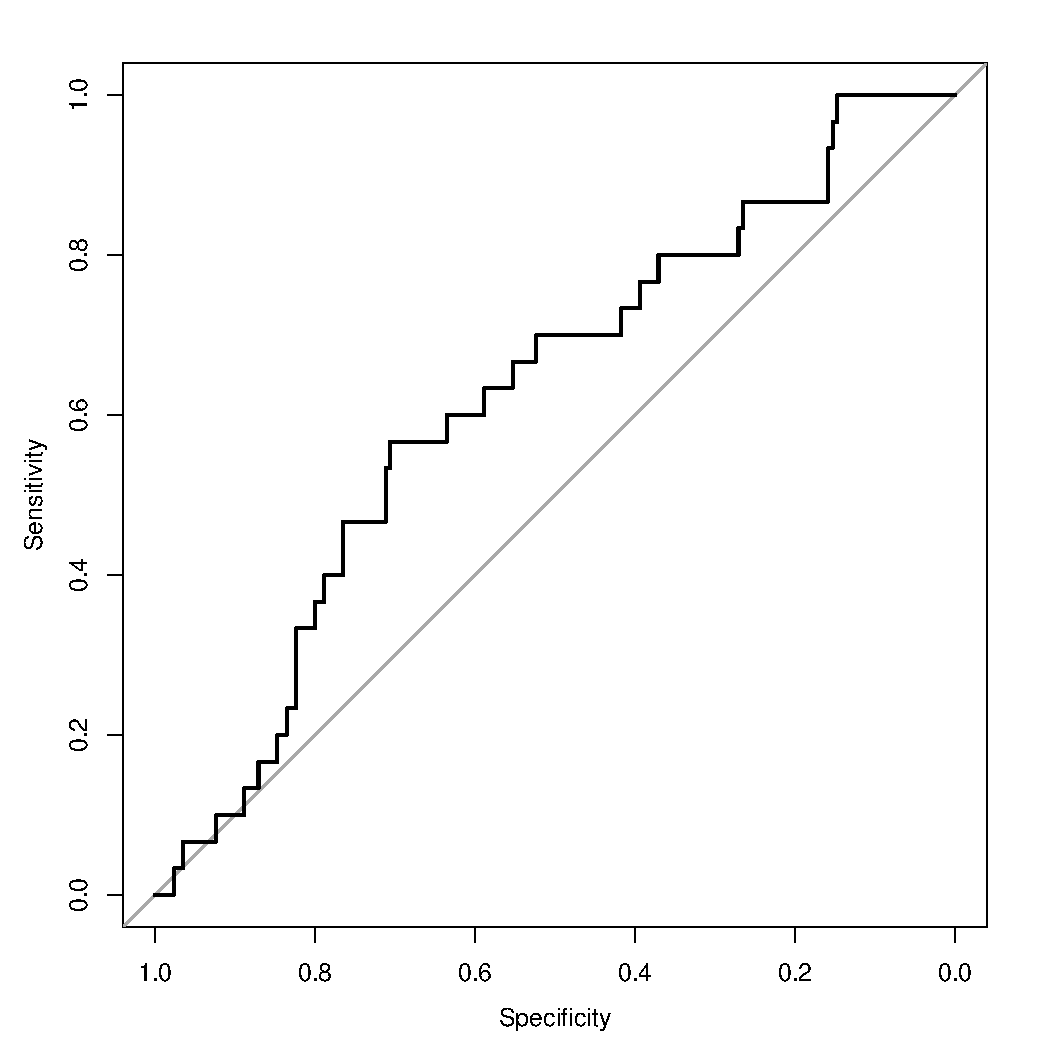
\includegraphics[width=\maxwidth]{figure/unnamed-chunk-17-1} 

\end{knitrout}

Adding another predictor helps improve the prediction:
\begin{knitrout}
\definecolor{shadecolor}{rgb}{0.969, 0.969, 0.969}\color{fgcolor}\begin{kframe}
\begin{alltt}
\hlstd{glmcoll1} \hlkwb{<-} \hlkwd{glm}\hlstd{(popcollapse}\hlopt{~}\hlstd{pheno_autocorr}\hlopt{+}\hlstd{variance,}
                \hlkwc{data} \hlstd{= decline,} \hlkwc{family} \hlstd{=} \hlstr{"binomial"}\hlstd{)}

\hlkwd{plot.roc}\hlstd{(}\hlkwc{predictor} \hlstd{=} \hlkwd{predict}\hlstd{(glmcoll1,} \hlkwc{type} \hlstd{=} \hlstr{"response"}\hlstd{),}
         \hlkwc{x} \hlstd{= decline}\hlopt{$}\hlstd{popcollapse)}
\end{alltt}
\end{kframe}
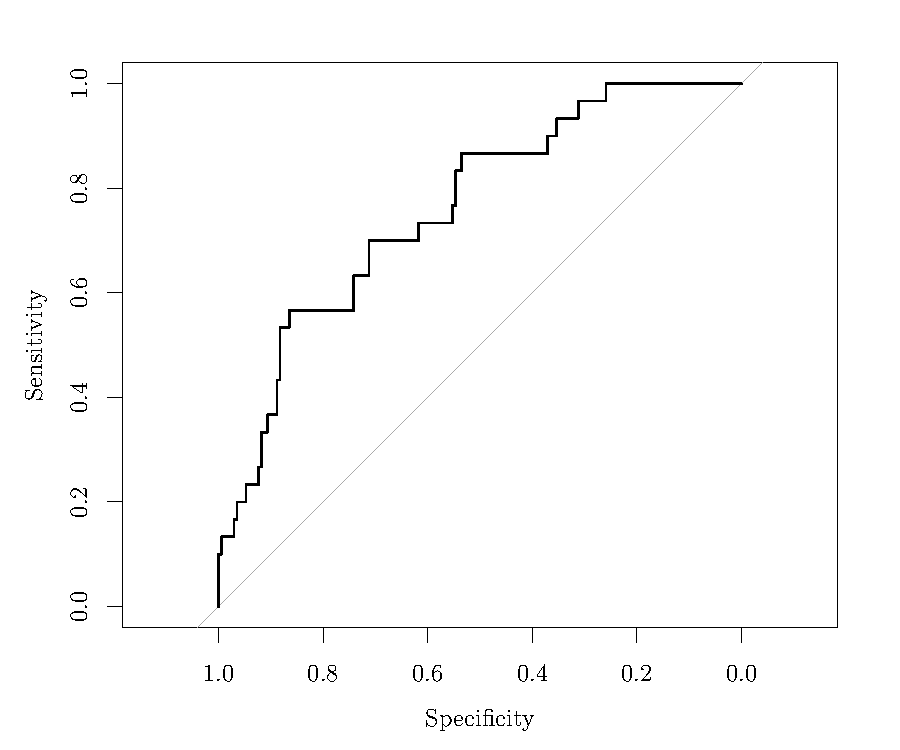
\includegraphics[width=\maxwidth]{figure/rocplot-1} 

\end{knitrout}

\end{Answer}



\section{Repeatability}



\begin{Exercise}[difficulty=2, title={Repeatability, on what scale?}]
Load the dataset \texttt{runaway.csv}. It contains fake data of a behavioural experiment: you played the trumpet to an animal and see whether it an animal and see whether they ran away. 500 individuals were tested twice a year during 5 years. You measured distance between you and the animal. You would like to know whether individuals behave consistently that is, have a personality and are repeatable. We start by fitting a linear mixed model using the package lme4 (accounting for differences among years, and for the effect of distance):
\begin{knitrout}
\definecolor{shadecolor}{rgb}{0.969, 0.969, 0.969}\color{fgcolor}\begin{kframe}
\begin{alltt}
\hlstd{roodat} \hlkwb{<-} \hlkwd{read.csv}\hlstd{(}\hlstr{"runaway.csv"}\hlstd{)}
\hlstd{lmm0} \hlkwb{<-} \hlkwd{lmer}\hlstd{(RunAway} \hlopt{~} \hlnum{1} \hlopt{+} \hlstd{distance} \hlopt{+}\hlstd{(}\hlnum{1}\hlopt{|}\hlstd{individual)} \hlopt{+} \hlstd{(}\hlnum{1}\hlopt{|}\hlstd{year),}
             \hlkwc{data} \hlstd{= roodat)}
\hlkwd{VarCorr}\hlstd{(lmm0)}
\end{alltt}
\begin{verbatim}
##  Groups     Name        Std.Dev.
##  individual (Intercept) 0.0663  
##  year       (Intercept) 0.0159  
##  Residual               0.4139
\end{verbatim}
\end{kframe}
\end{knitrout}
This model suggests a repeatability of:
\begin{knitrout}
\definecolor{shadecolor}{rgb}{0.969, 0.969, 0.969}\color{fgcolor}\begin{kframe}
\begin{alltt}
\hlstd{(}\hlnum{0.0663}\hlopt{^}\hlnum{2}\hlstd{)}\hlopt{/}\hlstd{(}\hlnum{0.0663}\hlopt{^}\hlnum{2}\hlopt{+}\hlnum{0.0159}\hlopt{^}\hlnum{2}\hlopt{+}\hlnum{0.4139}\hlopt{^}\hlnum{2}\hlstd{)}
\end{alltt}
\begin{verbatim}
## [1] 0.02498
\end{verbatim}
\end{kframe}
\end{knitrout}
That is not a lot, and we wonder whether the small number is due to the lack of fit of the model. Fortunately it is possible to fit a logistic mixed model by changing \texttt{lmer} to \texttt{glmer} and specifying \texttt{family=`binomial'}. If you do so, what repeatibility do you find? Where does the difference come from? What is right?
\end{Exercise}
\begin{Answer}
\begin{knitrout}
\definecolor{shadecolor}{rgb}{0.969, 0.969, 0.969}\color{fgcolor}\begin{kframe}
\begin{alltt}
\hlkwd{summary}\hlstd{(repmod} \hlkwb{<-} \hlkwd{glmer}\hlstd{(RunAway} \hlopt{~} \hlnum{1} \hlopt{+} \hlstd{distance} \hlopt{+}\hlstd{(}\hlnum{1}\hlopt{|}\hlstd{individual)} \hlopt{+}
                          \hlstd{(}\hlnum{1}\hlopt{|}\hlstd{year),} \hlkwc{data} \hlstd{= roodat,} \hlkwc{family} \hlstd{=} \hlstr{"binomial"}\hlstd{))}
\end{alltt}
\begin{verbatim}
## Generalized linear mixed model fit by maximum likelihood (Laplace
##   Approximation) [glmerMod]
##  Family: binomial  ( logit )
## Formula: RunAway ~ 1 + distance + (1 | individual) + (1 | year)
##    Data: roodat
## 
##      AIC      BIC   logLik deviance df.resid 
##     5354     5380    -2673     5346     4996 
## 
## Scaled residuals: 
##    Min     1Q Median     3Q    Max 
## -2.447  0.430  0.503  0.555  0.771 
## 
## Random effects:
##  Groups     Name        Variance Std.Dev.
##  individual (Intercept) 0.13740  0.3707  
##  year       (Intercept) 0.00513  0.0716  
## Number of obs: 5000, groups:  individual, 500; year, 5
## 
## Fixed effects:
##             Estimate Std. Error z value Pr(>|z|)    
## (Intercept)   1.7448     0.1189   14.67   <2e-16 ***
## distance     -0.1621     0.0347   -4.67    3e-06 ***
## ---
## Signif. codes:  0 '***' 0.001 '**' 0.01 '*' 0.05 '.' 0.1 ' ' 1
## 
## Correlation of Fixed Effects:
##          (Intr)
## distance -0.903
\end{verbatim}
\begin{alltt}
\hlkwd{VarCorr}\hlstd{(repmod)}
\end{alltt}
\begin{verbatim}
##  Groups     Name        Std.Dev.
##  individual (Intercept) 0.3707  
##  year       (Intercept) 0.0716
\end{verbatim}
\end{kframe}
\end{knitrout}

So the repeatability on the logit scale is:
\begin{knitrout}
\definecolor{shadecolor}{rgb}{0.969, 0.969, 0.969}\color{fgcolor}\begin{kframe}
\begin{alltt}
\hlnum{0.3707}\hlopt{^}\hlnum{2}\hlopt{/}\hlstd{(}\hlnum{0.0716}\hlopt{^}\hlnum{2}\hlopt{+}\hlnum{0.3707}\hlopt{^}\hlnum{2}\hlstd{)}
\end{alltt}
\begin{verbatim}
## [1] 0.964
\end{verbatim}
\end{kframe}
\end{knitrout}
That is much much higher than the LMM estimate (about 2\% versus about 96\%). 

This huge difference comes from two things: first, the logit transformation is not linear, and may distort variation. We can get a taste for that by back-transforming random numbers generated with the random effect variances and fixed effect coefficients. For instance, when \texttt{distance=3}, the repeatability on the back-transformed scale is approximately:

\begin{knitrout}
\definecolor{shadecolor}{rgb}{0.969, 0.969, 0.969}\color{fgcolor}\begin{kframe}
\begin{alltt}
\hlkwd{var}\hlstd{(}\hlnum{1}\hlopt{/}\hlstd{(}\hlnum{1}\hlopt{+}\hlkwd{exp}\hlstd{(}\hlopt{-}\hlstd{(}\hlkwd{rnorm}\hlstd{(}\hlnum{1000000}\hlstd{,} \hlnum{1.7448}\hlopt{-}\hlnum{0.1621}\hlopt{*}\hlnum{3}\hlstd{,} \hlnum{0.3707}\hlstd{)))))} \hlopt{/}
  \hlkwd{var}\hlstd{(}\hlnum{1}\hlopt{/}\hlstd{(}\hlnum{1}\hlopt{+}\hlkwd{exp}\hlstd{(}\hlopt{-}\hlstd{(}\hlkwd{rnorm}\hlstd{(}\hlnum{1000000}\hlstd{,} \hlnum{1.7448}\hlopt{-}\hlnum{0.1621}\hlopt{*}\hlnum{3}\hlstd{,} \hlnum{0.0716}\hlopt{+}\hlnum{0.3707}\hlstd{)))))}
\end{alltt}
\begin{verbatim}
## [1] 0.7006
\end{verbatim}
\end{kframe}
\end{knitrout}
That is a bit less, but not really small.

Also, notice that the repeatability is not the same for all values of \texttt{distance}:
\begin{knitrout}
\definecolor{shadecolor}{rgb}{0.969, 0.969, 0.969}\color{fgcolor}\begin{kframe}
\begin{alltt}
\hlkwd{var}\hlstd{(}\hlnum{1}\hlopt{/}\hlstd{(}\hlnum{1}\hlopt{+}\hlkwd{exp}\hlstd{(}\hlopt{-}\hlstd{(}\hlkwd{rnorm}\hlstd{(}\hlnum{1000000}\hlstd{,} \hlnum{1.7448}\hlopt{-}\hlnum{0.1621}\hlopt{*}\hlnum{0}\hlstd{,} \hlnum{0.3707}\hlstd{)))))} \hlopt{/}
  \hlkwd{var}\hlstd{(}\hlnum{1}\hlopt{/}\hlstd{(}\hlnum{1}\hlopt{+}\hlkwd{exp}\hlstd{(}\hlopt{-}\hlstd{(}\hlkwd{rnorm}\hlstd{(}\hlnum{1000000}\hlstd{,} \hlnum{1.7448}\hlopt{-}\hlnum{0.1621}\hlopt{*}\hlnum{0}\hlstd{,} \hlnum{0.0716}\hlopt{+}\hlnum{0.3707}\hlstd{)))))}
\end{alltt}
\begin{verbatim}
## [1] 0.685
\end{verbatim}
\begin{alltt}
\hlkwd{var}\hlstd{(}\hlnum{1}\hlopt{/}\hlstd{(}\hlnum{1}\hlopt{+}\hlkwd{exp}\hlstd{(}\hlopt{-}\hlstd{(}\hlkwd{rnorm}\hlstd{(}\hlnum{1000000}\hlstd{,} \hlnum{1.7448}\hlopt{-}\hlnum{0.1621}\hlopt{*}\hlnum{6}\hlstd{,} \hlnum{0.3707}\hlstd{)))))} \hlopt{/}
  \hlkwd{var}\hlstd{(}\hlnum{1}\hlopt{/}\hlstd{(}\hlnum{1}\hlopt{+}\hlkwd{exp}\hlstd{(}\hlopt{-}\hlstd{(}\hlkwd{rnorm}\hlstd{(}\hlnum{1000000}\hlstd{,} \hlnum{1.7448}\hlopt{-}\hlnum{0.1621}\hlopt{*}\hlnum{6}\hlstd{,} \hlnum{0.0716}\hlopt{+}\hlnum{0.3707}\hlstd{)))))}
\end{alltt}
\begin{verbatim}
## [1] 0.7115
\end{verbatim}
\end{kframe}
\end{knitrout}

The other important reason why repeatability is so much smaller in the LMM is that our GLMM does not explicitly measures the residual variation! For a logistic regression residual variance is not defined on the transformed scale, instead a Bernouilli random process generates deviations between a model prediction and data. The variation in this process is only a function of the expected probability.

To see what it does, lets draw random Bernouilli numbers around our expected back-transformed values before calculating the total variance:
\begin{knitrout}
\definecolor{shadecolor}{rgb}{0.969, 0.969, 0.969}\color{fgcolor}\begin{kframe}
\begin{alltt}
\hlkwd{var}\hlstd{(}\hlnum{1}\hlopt{/}\hlstd{(}\hlnum{1}\hlopt{+}\hlkwd{exp}\hlstd{(}\hlopt{-}\hlstd{(}\hlkwd{rnorm}\hlstd{(}\hlnum{1000000}\hlstd{,} \hlnum{1.7448}\hlopt{-}\hlnum{0.1621}\hlopt{*}\hlnum{3}\hlstd{,} \hlnum{0.3707}\hlstd{)))))} \hlopt{/}
  \hlkwd{var}\hlstd{(}\hlkwd{sapply}\hlstd{(}\hlkwc{X} \hlstd{=} \hlkwd{rnorm}\hlstd{(}\hlnum{100000}\hlstd{,} \hlnum{1.7448}\hlopt{-}\hlnum{0.1621}\hlopt{*}\hlnum{0}\hlstd{,} \hlnum{0.0716}\hlopt{+}\hlnum{0.3707}\hlstd{),}
        \hlkwc{FUN}\hlstd{=}\hlkwa{function}\hlstd{(}\hlkwc{x}\hlstd{)\{}\hlkwd{rbinom}\hlstd{(}\hlkwc{n} \hlstd{=} \hlnum{1}\hlstd{,} \hlkwc{size} \hlstd{=} \hlnum{1}\hlstd{,} \hlkwc{prob} \hlstd{=} \hlnum{1}\hlopt{/}\hlstd{(}\hlnum{1}\hlopt{+}\hlkwd{exp}\hlstd{(}\hlopt{-}\hlstd{(x))))}
                        \hlstd{\}))}
\end{alltt}
\begin{verbatim}
## [1] 0.0308
\end{verbatim}
\end{kframe}
\end{knitrout}

So, about 3\% of the data variation is explained by the individual random effect! That is not a perfectly exact calculation though, because it is only for the value of \texttt{distance=3}. To be exact we should integrate individual differences over the range of possible predictor values (that is a bit complicated).

The package QGglmm offers a proper back-transformation of variance components and repeatability on the data scale (denoted $h^2.obs$ below):
\begin{knitrout}
\definecolor{shadecolor}{rgb}{0.969, 0.969, 0.969}\color{fgcolor}\begin{kframe}
\begin{alltt}
\hlkwd{library}\hlstd{(QGglmm)}
\hlstd{QGglmm}\hlopt{::}\hlkwd{QGparams}\hlstd{(}\hlkwc{predict} \hlstd{=} \hlkwd{predict}\hlstd{(repmod),}\hlkwc{var.a} \hlstd{=} \hlnum{0.3707}\hlopt{^}\hlnum{2}\hlstd{,}
                 \hlkwc{var.p} \hlstd{=} \hlnum{0.0716}\hlopt{^}\hlnum{2}\hlopt{+}\hlnum{0.3707}\hlopt{^}\hlnum{2}\hlstd{,} \hlkwc{model} \hlstd{=} \hlstr{"binom1.logit"}\hlstd{)}
\end{alltt}
\begin{verbatim}
## [1] "Computing observed mean..."
## [1] "Computing variances..."
## [1] "Computing Psi..."
##   mean.obs var.obs var.a.obs  h2.obs
## 1   0.7671  0.1787  0.004095 0.02292
\end{verbatim}
\end{kframe}
\end{knitrout}

\end{Answer}
\end{document}
